% -*- coding: utf-8 -*-

\begin{chapter}{Исследовательское путешествие}\label{chap:1}
% \chapter{A Voyage of Discovery}
Влияние океана на погоду и климат часто обсуждается в новостях. Кто не слышал 
об Эль-Ниньо, изменении погоды, Атлантическом сезоне ураганов и штормовых 
%% изменении погоды --- weather patterns
нагонах? Однако, какую именно роль в этих процессах играет океан, и почему 
нас заботит подобный вопрос?
%
% The role of the ocean\index{ocean} on weather and climate is often discussed 
% in the news. Who has not heard of El Ni\~{n}o and changing weather patterns, 
% the Atlantic hurricane season and storm surges? Yet, what exactly is the 
% role of the ocean? And, why do we care?

\begin{section}{Зачем изучать физику океана?}
% \section[Physics of the ocean]{Why study the Physics of the ocean?}
Ответ зависит от наших интересов, которые, в свою очередь, определяются тем,
как мы используем океан. Следующие три аспекта имеют особую важность:
%
% The answer depends on our interests, which devolve from our use of the ocean. 
% Three broad themes are important:

\begin{itemize}
\item 
Океан~--- источник пищи. Поэтому мы интересуемся влияющими на него процессами 
так же, как фермеры~--- погодой и климатом. Океану не просто присущи 
некоторые погодные условия, такие как изменения температуры и течения; 
важность этих характеристик в том, что они определяют биологическую 
продуктивность моря. С другой стороны, атмосферные условия редко затрагивают 
плодородие почвы, за исключением разве что небольшого количества азота, 
фиксируемого молниями.
%
% \vitem We get food from the ocean. Hence we may be interested in processes 
% which influence the sea just as farmers are interested in the weather and 
% climate. The ocean not only has weather such as temperature changes and 
% currents, but the oceanic  weather fertilizes the sea. The atmospheric 
% weather seldom fertilizes fields except for the small amount of nitrogen 
% fixed by lightning.

\item
Океан используется человеком. Мы строим различные сооружения на побережье 
или просто в море, транспортируем грузы, добываем нефть и газ, а также 
отдыхаем: купаемся, катаемся на лодках, рыбачим, занимаемся серфингом 
и подводным плаванием. Таким образом, нам интересны процессы, которые 
влияют на эту деятельность, особенно волны, ветры, течения и температура.
%
% \vitem We use the ocean. We build structures on the shore or just offshore. 
% We use the ocean for transport. We obtain oil and gas below the ocean. 
% And, we use the ocean for recreation, swimming, boating, fishing, surfing,
% and diving. Hence we are interested in processes that influence these
% activities, especially waves, winds, currents, and temperature.

\item
Океан влияет на погоду и климат: распределение дождей, засух, 
наводнений, региональный климат и развитие штормов, ураганов и тайфунов. 
Следовательно, нам интересно взаимодействие океана с атмосферой, 
особенно потоки тепла и воды, проходящие через поверхность моря, 
транспорт тепла океанами, а также их влияние на климат и синоптическую 
ситуацию.
%
% \vitem The ocean influence the atmospheric weather and climate. The ocean 
% influence the distribution of rainfall, droughts, floods, regional climate, 
% and the development of storms, hurricanes, and typhoons. Hence we are 
% interested in air-sea interactions, especially the fluxes of heat and water 
% across the sea surface, the transport of heat by the ocean, and the influence 
% of the ocean on climate and weather patterns.
\end{itemize}

Эти темы влияют на выбор объектов изучения. Объекты определяют, что мы меряем, 
как производим измерения и где. Некоторые процессы локальны, такие как 
разрушение волн на пляже, некоторые~--- региональны, такие как влияние севера 
Тихого океана на погоду Аляски, а некоторые~--- глобальны, такие как влияние 
океанов на изменение климата и глобальное потепление.
%
% These themes influence our selection of topics to study. The topics then
% determine what we measure, how the measurements are made, and the geographic 
% areas of interest. Some processes are local, such as the breaking of waves 
% on a beach, some are regional, such as the influence of the North Pacific on 
% Alaskan weather, and some are global, such as the influence of the ocean on 
% changing climate and global warming.  
 
Если эти причины для изучения океана действительно важны, давайте начнём 
наше исследовательское путешествие. Любому путешествию необходим пункт 
назначения. Какой же следует избрать нам?
%
% If indeed, these reasons for the study of the ocean are important, lets
% begin a voyage of discovery. Any voyage needs a destination. What is ours?
\end{section}

\begin{section}{Цели}
% \section{Goals}
В целом, я надеюсь, что студенты почерпнут из этого учебника
представление о главных концептуальных схемах (или теориях) физической 
океанографии, лежащих в её основе, о том, какой путь в процессе их построения 
довелось пройти науке, а также о причинах их широкого признания. Помимо этого 
мы познакомимся с методами, которыми океанографы извлекают закономерности из
океана случайностей, и рассмотрим роль эксперимента в океанографии
(перефразируя~\cite[стр.~89]{Shamos:1995}).
%
% At the most basic level, I hope you, the students who are reading this text, 
% will become aware of some of the major conceptual schemes (or theories) that 
% form the foundation of physical oceanography\index{physical oceanography!goals of}, 
% how they were arrived at, and why they are widely accepted, how oceanographers 
% achieve order out of a random ocean, and the role of experiment in 
% oceanography (to paraphrase Shamos, 1995: p. 89).

В частности, я ожидаю, что читательская аудитория будет в итоге способна 
описать физические процессы, происходящие в океанах и прибрежных зонах, 
взаимодействие океана и атмосферы, распределение океанских ветров, течений, 
потоков тепла и водных масс. В тексте общим идеям уделено большее внимание, 
чем математическим выкладкам. Мы постараемся ответить на следующие вопросы:
%
% More particularly, I expect you will be able to describe physical processes 
% influencing the ocean and coastal regions: the interaction of the ocean with 
% the atmosphere, and the distribution of oceanic winds, currents, heat 
% fluxes\index{heat flux}, and water masses. The text emphasizes ideas rather 
% than mathematical techniques. I will try to answer such questions as:

\begin{enumerate}
\item
Какова основа нашего понимания физики океана?
%
% What is the basis of our understanding of physics of the ocean?

\begin{itemize}
  \item
  Что такое физические свойства морской воды? 
%
% \item What are the physical properties of sea water?

  \item
  Каковы важные термодинамические и динамические процессы, влияющие на океан? 
%
% \item What are the important thermodynamic and dynamic processes influencing 
% the ocean?

  \item
  Какие уравнения описывают эти процессы, и как они выведены? 
%
% \item What equations describe the processes and how were they derived?

  \item
  Какие допущения мы использовали для их вывода? 
%
% \item What approximations were used in the derivation?

  \item
  Имеют ли эти уравнения полезные решения? 
%
% \item Do the equations have useful solutions?

  \item
  Насколько хорошо эти решения описывают процесс? То есть, каковы 
  экспериментальные основания теорий? 
%
% \item How well do the solutions describe the process? That is, what is the
% experimental basis for the theories?

  \item
  Какие процессы плохо понятны? Какие~--- хорошо?
%
% \item Which processes are poorly understood? Which are well understood?
\end{itemize}

\item
Каковы источники информации о физических переменных?
%
% \item What are the sources of information about physical variables?

\begin{itemize}
  \item
  Какие инструменты используются для измерения каждой переменной? 
%
% \item What instruments are used for measuring each variable?

  \item
  Каковы их точность и ограничения? 
%
% \item What are their accuracy and limitations?

  \item
  Какие данные существуют за длительный период времени? 
%
% \item What historic data exist?

  \item
  Какая платформа используется: cпутники, корабли, буи, буйковые станции?
%
% \item What platforms are used? Satellites, ships, drifters\index{drifters}, 
% moorings?
\end{itemize}

\item
Какие процессы важны? Некоторые важные процессы, которые мы будем изучать, 
включают:
%
% What processes are important? Some important process we will study include:
\begin{itemize}
  \item
  накопление и транспорт тепла в океанах;
%
% \item Heat storage and transport \index{transport!heat}in the ocean.

  \item
  обмен теплом с атмосферой и роль океана в климате; 
%
% \item The exchange of heat with the atmosphere and the role of the ocean 
% in climate.

  \item
  ветровое и температурное воздействие на поверхностный слой перемешивания; 
%
% \item Wind and thermal forcing of the surface mixed 
% layer\index{mixed layer!external forcing of}.

  \item
  ветровую циркуляцию (включая экмановский перенос, экмановскую подкачку
%% "Экмановская циркуляция" и "Экмановский насос" в русском переводе "Динамики
%% атмосферы и океана" А. Гилла называется "экмановский перенос" и "экмановская 
%% подкачка" соотв.?
  глубинной циркуляции, а также апвеллинг). 
%
% \item The wind-driven circulation including the Ekman circulation, Ekman 
% pumping\index{Ekman pumping} of the deeper circulation, and 
% upwelling\index{upwelling!due to Ekman pumping}.

  \item
  динамику океанических течений (в частности, геострофические течения и роль 
  завихренности); 
%
% \item The dynamics of ocean currents, including 
% geostrophic\index{geostrophic currents} currents and the role of vorticity.

  \item
  формирование типов воды и водных масс;
%
% \item The formation of water types\index{water!type} and masses.

  \item
  глубинную циркуляцию океана; 
%
% \item The deep circulation of the ocean.

  \item
  экваториальную динамику, Эль-Ниньо и влияние океана на погоду; 
%
% \item Equatorial dynamics, El Ni\~{n}o, and the role of the ocean in weather.

  \item
  математические модели циркуляции; 
%
% \item Numerical models of the circulation.
  \item
  волны в океане (в том числе поверхностные волны, инерционные колебания, 
  приливы и цунами); 
%
% \item Waves in the ocean including surface waves, inertial
% oscillations\index{inertial!oscillation}, tides, and tsunamis\index{tsunami}.

  \item
  волны в мелкой воде, прибрежные процессы и предсказание приливов.
%
% \item Waves in shallow water, coastal processes, and tide predictions.
\end{itemize}

\item
Каковы основные течения и водные массы в океане, что определяет их 
распределение?
%
% \item What are a few of the major currents and water masses in the ocean,
% and what governs their distribution?
\end{enumerate}
\end{section}

\begin{section}{Организация (структура)}
% \section{Organization}
Перед тем, как начать путешествие, мы обычно стараемся узнать о тех местах, 
которые собираемся посетить, для чего изучаем карты и путеводители. 
В нашей книге путеводителями будут статьи и книги, написанные океанографами. 
Мы начнем с краткого обзора того, что известно об океанах. 
Затем продолжим описанием океанских бассейнов, чтобы понять, как форма 
морей влияет на физические процессы в воде. Далее мы рассмотрим внешние силы, 
ветер и тепло, действующие на океан, и его отклик на них. Во время изучения 
будут изложены необходимые теоретические сведения и представлены натурные 
данные.
%
% Before beginning a voyage, we usually try to learn about the places we will
% visit. We look at maps and we consult travel guides. In this book, our guide 
% will be the papers and books published by oceanographers. We begin with a 
% brief overview of what is known about the ocean. We then proceed to a 
% description of the ocean basins, for the shape of the seas influences the 
% physical processes in the water. Next, we study the external forces, wind 
% and heat, acting on the ocean, and the ocean's response. As we proceed, 
% I bring in theory and observations as necessary.


К тому времени, когда мы достигнем главы 7, нам необходимо будет понять 
уравнения, описывающие динамическую реакцию океана. Так, мы рассмотрим 
уравнения движения, влияние вращения Земли и вязкости. Это приведёт к 
изучению ветровых океанических течений, геострофического приближения и важности 
постоянства вихря.
%
% By the time we reach chapter 7, we will need to understand the equations 
% describing dynamic response of the ocean. So we consider the equations of 
% motion, the influence of earth's rotation, and viscosity. This leads to a 
% study of wind-driven ocean currents, the geostrophic 
% approximation\index{geostrophic approximation}, and the usefulness of 
% conservation of vorticity.

В дальнейшем мы обсудим некоторые частные примеры: глубинную циркуляцию, 
экваториальный океан и Эль-Ниньо, а также циркуляцию отдельных частей океана. 
Затем рассмотрим роль математического моделирования в описании океана. 
В завершение мы изучим прибрежные процессы, волны, приливы, предсказание волн 
и приливов, цунами и штормовые нагоны.
%
% Toward the end, we consider some particular examples: the deep circulation, 
% the equatorial ocean and El Ni\~{n}o, and the circulation of particular areas 
% of the ocean. Next we look at the role of numerical models in describing 
% the ocean. At the end, we study coastal processes, waves, tides, wave and 
% tidal forecasting, tsunamis\index{tsunami}, and storm surges.
\end{section}

\begin{section}{Общая картина}
% \section{The Big Picture}
Океан представляет собой одну из частей географической оболочки. 
Он оказывает влияние на атмосферные процессы путем переноса массы, момента и
энергии через водную поверхность. Речной сток, вместе с растворёнными в нем
минеральными веществами, тоже в конечном итоге оказывается в океане. 
Накопленные осадочные материалы со временем становятся скальной
породой на суше. Следовательно, понимание океана важно для получения картины 
всей Земли как системы в целом, так и вопросов глобальной смены климата и
%% important problems such as global change or global warming
%% из контекста не вполне ясно, о каком "изменении" идет речь
глобального потепления в частности. На более общем уровне, физическая 
океанография и метеорология сближаются. Океан обеспечивает обратную связь,
замедляющую изменения в состоянии атмосферы.
%
% The ocean is one part of the earth system. It mediates processes in the 
% atmosphere by the transfers of mass, momentum, and energy through the sea 
% surface. It receives water and dissolved substances from the land. And, it 
% lays down sediments that eventually become rocks on land. Hence an 
% understanding of the ocean is important for understanding the earth as a 
% system, especially for understanding important problems such as global change 
% or global warming. At a lower level, physical oceanography and meteorology 
% are merging. The ocean provides the feedback leading to slow changes in 
% the atmosphere.

Я надеюсь, вы обратите внимание на то, что при описании динамики океана мы 
будем использовать теорию, натурные (эмпирические) данные и численные модели. 
Их необходимо рассматривать вместе, по отдельности они не самодостаточны.
%
% As we study the ocean, I hope you will notice that we use theory,
% observations, and numerical models to describe ocean dynamics.
% \index{physical oceanography!big picture} \textit{None is sufficient by 
% itself}.

\begin{enumerate}
\item
Процессы в океане нелинейны и турбулентны, а теория нелинейных, турбулентных 
потоков в сложных бассейнах не очень хорошо развита. Теории, используемые 
для описания океана~--- сильно упрощённые приближения реальности. 
%
% \vitem Ocean processes\index{ocean!processes in} are nonlinear and turbulent. 
% Yet we don't really understand the theory of non-linear, turbulent flow 
% in complex basins. Theories used to describe the ocean are much simplified 
% approximations to reality.

\item
Натурные измерения разбросаны в пространстве и во времени. Они обеспечивают 
грубое описание усреднённого по времени потока, но большинство процессов 
во многих регионах ещё мало исследованы.
%
% \vitem Observations\index{observations} are sparse in time and space.
% They provide a rough description of the time-averaged flow, but many
% processes in many regions are poorly observed.

\item
Численные модели включают наиболее реалистичные теоретические идеи, они могут 
помочь интерполировать натурные исследования во времени и пространстве 
и используются для предсказания климатических изменений, течений и волн. 
Однако, численные равенства являются приближениями непрерывных аналитических 
уравнений, описывающих жидкий поток; они не содержат никакой информации о 
потоке между узловыми точками, в силу чего пока не могут использоваться 
для полного описания турбулентного потока, наблюдающегося в океане. 
%
% \item Numerical models\index{numerical models} include much-more-realistic 
% theoretical ideas, they can help interpolate oceanic observations in time 
% and space, and they are used to forecast climate change, currents, and waves.
% Nonetheless, the numerical equations are approximations to the continuous 
% analytic equations that describe fluid flow, they contain no information
% about flow between grid points, and they cannot yet be used to describe 
% fully the turbulent flow seen in the ocean.
\end{enumerate}

Соединяя теорию и натурные измерения в численных моделях, мы избегаем 
сложностей, связанных с их использованием по отдельности 
(рис.~\ref{fig:bigpicture}). Способы комбинирования
этих подходов непрерывно совершенствуются, что ведёт к гораздо 
более точному описанию океана. Конечная цель~--- узнать океан так хорошо, 
чтобы можно было предсказывать будущие перемены в окружающей среде, 
включая изменения климата или реакцию рыбных ресурсов на перелов.
%
% By combining theory and observations in numerical models we avoid some of 
% the difficulties associated with each approach used separately (figure 1.1). 
% Continued refinements of the combined approach are leading to 
% ever-more-precise descriptions of the ocean. The ultimate goal is to know 
% the ocean well enough to predict the future changes in the environment, 
% including climate change or the response of fisheries to over fishing.

\begin{figure}[h!]
\makebox[121mm] [c]{\includegraphics{pics/bigpicture}}
\caption{Данные, численные модели и теория~--- все это необходимо для
понимания океана. В конечном итоге, понимание устройства системы 
<<океан-атмосфера-суша>> должно привести к возможности предсказывать 
ее будущее состояние.}
\label{fig:bigpicture}
\end{figure}
%
% \begin{figure}[h!]
% \makebox[121mm] [c]{\includegraphics{bigpicture}} 
% \footnotesize
% Figure 1.1 Data, numerical models, and \rule{0mm}{4ex}theory are
% all necessary to understand the ocean. Eventually, an
% understanding of the ocean-atmosphere-land system will lead to
% predictions of future states of the system.
% 
% \label{fig:bigpicture}
% \vspace{-1ex}
% \end{figure}


Объединение теории, натурных исследований и компьютерных моделей относительно 
молодо. Четыре десятилетия экспоненциального роста вычислительной мощности
привели к появлению массово доступных настольных компьютеров, способных 
моделировать важные физические процессы и динамику океана.
%
% The combination of theory, observations, and computer 
% models\index{numerical models} is relatively new. Four decades of exponential 
% growth in computing power has made available desktop computers capable 
% of simulating important physical processes and oceanic dynamics.

\begin{quotation}
Все мы, люди науки, знаем, что компьютер стал важнейшим исследовательским 
инструментом~\dots{} научные расчёты достигли того уровня, на котором 
они становятся инструментом научных и инженерных изысканий наравне
с лабораторным экспериментом и математической теорией.~\cite{Langer:1999}
%
% All of us who are involved in the sciences know that the computer has 
% become an essential tool for research \dots scientific computation has 
% reached the point where it is on a par with laboratory experiment and 
% mathematical theory as a tool for research in science and 
% engineering---Langer (1999).
\end{quotation}

Объединение теории, натурных исследований и компьютерных моделей предполагает 
новый путь развития океанологии. В прошлом океанограф должен был бы сформулировать 
теорию, собрать данные для её проверки, а затем опубликовать результаты. 
Теперь задачи стали настолько специализированными, что мало кто может всё 
это проделать в одиночку. Немногие преуспели одновременно в построении теорий, 
сборе данных и разработке численных моделей. Вместо этого всё больше и больше 
работы делается командами учёных и инженеров.
%
% The  combination of theory, observations, and computer models also
% implies a new way of doing oceanography\index{oceanography!new methods of}. 
% In the past, an oceanographer would devise a theory, collect data to test 
% the theory, and publish the results. Now, the tasks have become so 
% specialized that few can do it all. Few excel in theory, collecting data, 
% and numerical simulations. Instead, the work is done more and more by teams 
% of scientists and engineers.
\end{section}

\begin{section}{Дополнительная литература}
% \section{Further Reading}
Если вы знаете об океанах и океанографии не слишком много, я предлагаю 
вам начать с книги Маклениша, особенно её четвёртой главы, посвящённой 
<<чтению океана>>. 
%% Маклениша --- MacLeish ???
%% MacLeish's book, especially his Chapter 4 on "Reading the ocean
По моему мнению, в ней даётся наиболее полное нетехническое описание того, 
как океанографы идут к пониманию океана.
%
% If you know little about the ocean and oceanography, I suggest you begin by
% reading MacLeish's (1989) book \textit{The Gulf Stream\index{Gulf Stream}: 
% Encounters With the Blue God}, especially his Chapter 4 on ``Reading the 
% ocean.'' In my opinion, it is the best overall, non-technical, description 
% of how oceanographers came to understand the ocean.

Вы также можете извлечь немало полезных сведений из соответствующих глав любой 
океанографической книги начального уровня. Особый интерес представляют работы 
таких авторов, как Gross, Pinet, или Segar. Три публикации Открытого 
Университета, включенные в список литературы, ориентированы на более 
подготовленного читателя. 
%
% You may also benefit from reading pertinent chapters from any introductory 
% oceanographic textbook. Those by Gross, Pinet, or Segar are especially 
% useful. The three texts produced by the Open University provide a slightly 
% more advanced treatment.

\begin{itemize}
\item
Gross, M. Grant and Elizabeth Gross (1996) \textit{Oceanography, 
A View of Earth.} 7th edition. Prentice Hall.
%
% \item[Gross,] M. Grant and Elizabeth Gross (1996) \textit{Oceanography---A 
% View of Earth.} 7th edition. Prentice Hall.

\item
MacLeish, William (1989) \textit{The Gulf Stream: Encounters With the Blue God.}
Houghton Mifflin Company. 
%
% \item[MacLeish,] William (1989) \textit{The Gulf Stream: Encounters With
% the Blue God.} Houghton Mifflin Company.

\item
Pinet, Paul R. (2006) \textit{Invitation to Oceanography.} 4nd edition.
Jones and Bartlett Publishers.
%
% \item[Pinet,] Paul R. (2006) \textit{Invitation to Oceanography.} 4nd edition. 
% Jones and Bartlett Publishers.

\item
Open University (2001) \textit{Ocean Circulation.} 2nd edition. Pergamon Press.
%
% \item[Open University] (2001) \textit{Ocean Circulation.} 2nd edition. 
% Pergamon Press.

\item
Open University (1995) \textit{Seawater: Its Composition, Properties 
and Behavior.} 2nd edition. Pergamon Press.
%
% \item[Open University] (1995) \textit{Seawater: Its Composition, Properties 
% and Behavior.} 2nd edition. Pergamon Press.

\item
Open University (1989) \textit{Waves, Tides and Shallow-Water Processes.} 
Pergamon Press. 
%
% \item[Open University] (1989) \textit{Waves, Tides and Shallow-Water 
% Processes.} Pergamon Press.

\item
Segar, Douglas A. (2007) \textit{Introduction to Ocean Sciences.}
2nd edition. W. W. Norton.
%
% \item[Segar,] Douglas A. (2007) \textit{Introduction to Ocean Sciences.}
% 2nd edition. W. W. Norton.
\end{itemize}
\end{section}

\end{chapter}
